\documentclass[a4paper,12pt,titlepage]{article}

\usepackage{cite, amsmath}
% fonts
\usepackage{times}
\usepackage{latexsym}
% math symbols 
\usepackage{amsmath}
\usepackage{amssymb}
% for algorithms
\usepackage[ruled,vlined]{algorithm2e}  	% For algorithms
% for enumerations
\usepackage{enumerate}
%\usepackage{slashbox, extarrows}
% for inclusion of graphics
\usepackage{graphicx}
% wrap figures with text
\usepackage{wrapfig}
% include eps-files 
\usepackage{epsfig}
% boxing for a minipage
\usepackage{boxedminipage}
% to make sure \includegraphics works with eps-files 
% when using LATEX => PDF compilation
\usepackage{epstopdf}
% pgfplots for the graphs
\usepackage{pgfplots}
% verbatin for easy text formatted teletype like short program code 
\usepackage{verbatim}
% for URLs -- has some issues when activating URLs that contain special characters, e.g., space and tilde. 
% \usepackage{url}
% for hyperrefs -- resolves the above problem of the url package and adds dynamic linking within the final pdf document 
% that is visualized correctly both in digital and printed form. 
\usepackage{hyperref}
% for good looking tables
\usepackage{supertabular}	
% tables with multirow
\usepackage{multirow}
\usepackage{todonotes}

\makeatletter
\newcommand\subsubsubsection{\@startsection{paragraph}{4}{\z@}%
            {-2.5ex\@plus -1ex \@minus -.25ex}%
            {1.25ex \@plus .25ex}%
            {\normalfont\normalsize\bfseries}}
\makeatother
\setcounter{secnumdepth}{4} % how many sectioning levels to assign numbers to
\setcounter{tocdepth}{4}    % how many sectioning levels to show in ToC

% set the margins 
\usepackage[top=1.5in, bottom=1.5in, left=1.2in, right=1.2in]{geometry}
\usepackage[utf8]{inputenc}
\usepackage[british,UKenglish,USenglish,american]{babel}
\usepackage{fancyhdr}
\usepackage{fancyref}
\usepackage{caption}
\usepackage{apacite}
\usepackage{subcaption}
\usepackage{gensymb}
\usepackage[nottoc]{tocbibind}

\renewcommand*{\reftextfaceafter}{\unskip}
\renewcommand*{\reftextafter}{\unskip}
\renewcommand*{\reftextfacebefore}{\unskip}
\renewcommand*{\reftextbefore}{\unskip}
\makeatletter
\let\saved@reftextfaraway\reftextfaraway
\renewcommand*{\reftextfaraway}[1]{%
  \begingroup
    \def\ref@unknown@value{??}%
    \ifx\@tempa\ref@unknown@value
      \count@=0 %
    \else
      \count@\thevpagerefnum\relax
      \advance\count@ by -\@tempa\relax
      \ifnum\count@<0 \count@=-\count@\fi
    \fi
    \ifnum\count@<3 %
      \unskip
    \else
      \saved@reftextfaraway{#1}%
    \fi
  \endgroup
}
\makeatother

\usepackage{float}
\usepackage{tabto}
\usepackage{natbib}
\usepackage{amsmath,tabu}
\usepackage{setspace}

% for definition of custom floats as the float Code bellow
\usepackage{float} 
\floatstyle{ruled}
\newfloat{code}{thp}{lop}
\floatname{code}{Code}

\newenvironment{packed_enum}{
%\vspace{-1em}
\begin{enumerate}
  \setlength{\itemsep}{1pt}
  \setlength{\parskip}{0pt}
  \setlength{\parsep}{0pt}
}{\end{enumerate}
%\vspace{-1em}
}

\newenvironment{packed_enum_roman}{
\renewcommand{\labelenumi}{(\roman{enumi})}
%\vspace{-1em}
\begin{enumerate}
  \setlength{\itemsep}{1pt}
  \setlength{\parskip}{0pt}
  \setlength{\parsep}{0pt}
}{\end{enumerate}
%\vspace{-1em}
}

\newenvironment{packed_item}{
%\vspace{-1em}
\begin{itemize}
  \setlength{\itemsep}{1pt}
  \setlength{\parskip}{0pt}
  \setlength{\parsep}{0pt}
}{\end{itemize}
%\vspace{-1em}
}

% define the title




\title{

\includegraphics[width=0.4\textwidth]{KTH_eng_CMYK.eps} \\[1cm] User-centric Web-based System for Automatic Optimal Visualization of Geospatial Information \\
}
\author{Ella Syk \\ 
Fredrik Hilding \\ \\
Supervised by \\
Axel Bronder \\
Gy\H oz\H o Gid\'ofalvi \\ \\
Division of Geodesy and Geoinformatics\\
Department of Urban Planning and Environment\\
KTH Royal Institute of Technology}
\date{Stockholm 2016}

\begin{document}
\pagenumbering{gobble}
\maketitle
\begin{abstract}
%\boldmath  
test
\end{abstract}
\newpage
\section*{Acknowledgments}
\phantomsection
\addcontentsline{toc}{section}{\protect Acknowledgments}{}%
We would like to thank...
\newpage
\tableofcontents
\pagenumbering{Roman}
\newpage
\listoffigures
\newpage
\listoftables
\newpage
\section*{Terms and Abbreviations}
\begin{description}
\item [Ant] Ant-i
\item [Elephant] El Ephant
\end{description}

\newpage

\section{Introduction}
%MUUUUU

Today, interactive maps are part of our everyday lives since they reside on our phones and in public spaces, among many other places. Maps are now a base for many applications and are easily accessible on the web and part of other visualization tools as an interface to geographic information. Furthermore, many professionals in an assortment of different fields use them as the front of their information systems and perform map interpretations and spatial queries that previously were reserved for GIS analysts and cartographers.

One aspect that has surely aided in spreading interactive maps throughout professions and our culture is that they are so easily accessible and can be made location-aware, web based and even mobile compatible.

\pagenumbering{arabic}

\subsection{Background}

\subsection{Problem statement / research question}

All this boils down to a single research question: \textbf{ How can large and complex geospatial datasets best be presented for layman GIS-users?} This question is best answered by answering three sub questions:

\begin{itemize}
  \item Which techniques are suitable for a the building blocks of a NIS?  i.e. arcs and nodes
  \item How much of the analysis part can be automatized and how much of it still requires user guidance and input.
\end{itemize}

\subsection{Objectives}

\begin{itemize}
  \item Create a web-based solution for presentation and analysis of data, where tools and visualization techniques are tailored to the needs and level of the user.
  \item Draw general conclusions about the efficacy of different visualization techniques, as well as other areas, for layman GIS-users.
\end{itemize}


\subsection{Structure of the report(?)}

1) the general context of the problem \\ 
2) a brief description of the problem and its importance \\
3) a brief statement about why previously proposed approaches are not adequate \\
4) an outline of (the main ideas / steps / characteristics of) the proposed approach / method to the problem \\
5) a list of contributions potentially including evaluation and comparison of methods \\
6) a road map over the remaining sections of the documents. \\

\section{Related Work}
%Källorna måste fixas till - Ella}

\subsection{Visual Analytics}

Even today there is still no obvious generalized solution that provides the answer to how you should present your data, no matter if it is georeferenced or not. How to present your data in a smart and comprehensive way is still an everyday challenge. This is because presenting data involves several complex components that needs to be considered in order to provide a satisfactory presentation of the data. \citep{Andrienko}

Key features of visual analytics are data analysis, problem solving and decision-making, active involvement of a human in the analytical process and support for communication of analytical results to relevant recipients. Not only is the combination of these features complex to evaluate but all of these features are also complex in themselves. For instance they are hierarchical (different levels of abstraction can be seen) and multivariate with different properties. \citep {VisMaster}

Existing solutions often require significant expertise and are not very intuitive. There is a need for flexibility, the possibility to adjust the level of abstraction (actual data or aggregated data) and how the data is represented on the screen. Both experts and unaccustomed users would benefit from this flexibility, although the non expert may also require some guidance in choosing appropriate tools and visualization methods for their task. So one of the challenges is to determine when to use automated techniques or techniques involving a human in the analyst process. This means that when developing a new system involving visual analytics the developer has to know which techniques to choose for a given problem. The users in turn need to select a system, setting or method and therefore need information to make the appropriate decision in order to avoid wrong results. \citep {VisMaster}

There is a need to develop scientifically sound methods that can combine algorithmic processing with interactive visual interfaces, i.e. a semi-automated approach that allows human judgement to be involved in the analysis. Visual analytics differ from standard analysis approaches in the sense that it is based on the assumption that interactive visual representations can enhance human capability to establish links making inferences. \citep{Andrienko} Another aspect to consider is that in visual analytics new data can arrive during the analysis. A semi-automated approach is required since visual analytics involves combinations large amounts of of complex data which requires reduction via automated methods. \citep {VisMaster}


\newpage
\subsection{GIS-Users}

With recent technological advancements in web- and mobile GIS, there has been a rapid increase in the amount of available applications, programs and services that deploy some kind of GIS technologies. \citep{VisMaster} Accompanying this rapid expansion of available technologies, there has also been a sizeable increase in the user base of these technologies. In the VisMaster project, they take this argument as far as to claim that virtually everybody is a spatio-temporal analyst in some way, shape or form. \citep{VisMaster}

However, the rapid increase of the user base is not without its problems. Previously, the spatio-temporal analysts were a small professional group, usually with special training in the field. The applications were designed for users expected to have a certain level of proficiency and knowledge of the GIS domain. \citep[p. 83]{VisMaster} Although these new users can be expected to possess a certain level of computer skills, their ability to not just access, but gain insight and knowledge from the geospatial data will depend on its presentation. \%inte nöjd med den sista meningen
%^Eventuellt annan källa? Andrienko? KTHs system nere, revidera senare

In recent years the evaluation and refinement of geovisualization software and GIS applications has become an important research topic. A consistent recommendation in the line of this research is placement of an early and active focus of the needs and expectations of the targeted end users during design and development i.e. user-centered design. \citep{CrimeAnalysis} The established GIS software developer Esri concurs with this notion and in their system design guidelines they state that “client participation is a key ingredient in the design process”, although traditionally the user needs assessment and the system architecture design has been two separate efforts \citep[pp. 1.4-6]{EsriReport} %Vilken sida?
However, since the user base today is so large and diverse this is not a trivial task and there is not much research on the topic.

%Another challenge regarding user groups is to determine how to conceptualize “expertise”. 


\subsection{Visualization}

As \citet{UserCenterApproach} states “humans have remarkable perceptual capabilities that tend to be underestimated in current visualization designs”. The reason for this is often due to the fact that it is often overlooked  who the users are, what tasks they aim to accomplish using the visualizations and what environments they work in. These are important factors since in order for the visualization to be considered successful the visualization must meet its goal which is to provide the user with a satisfactory experience. A good visualization for one user may be useless for another. Therefore it is essential that interactive visualization systems are designed for both specific tasks and specific types of users. \citep{UserCenterApproach}


%FÄRGBLINDHET

\subsubsection{Web Visualization}
The current GIS software is often large and complex since it is designed for performing different kinds of heavy analysis. This means there is access to many tools and operations that has purposes and uses which may not be obvious for the inexperienced user. %Nämn också att presentation av data knepigt för att brygga över till nästa stycke

One way to lower the threshold into the geospatial analyst world, is to make the data both easier to interpret, but also easier to access. One of the current leading research centers in the visualization and geospatial analytics field is NVIS, the Norrköping Visualization and Interaction Studio. In 2011, a study was performed where they transformed the functionality of an existing software from standalone to web-based. They sum up the status of the previous work as "...the benefits of geovisual analytics tools are many, it has been a challenge to adapt these tools to the Internet and reach a broader user community". \citep{WebEnabled} 

With  the rapid growth of the web, a number of different web browsers have also been created. Although supporting all of them is very difficult, any credible web GIS solution has to support the most commonly used, such as Safari, Internet Explorer, Firefox and Chrome. \citep{webGIS} 

There are of course also demands on the map itself from a visualization point of view. The Swedish Standards Institute (SIS) have been working on a technical report regarding standardizing guidelines for Web Map Services (WMS). In their report they state that WMS should offer a number of different map layers for presentation of the same object type. In practice this means that the user should be able to select different combinations of layers so that the object in contrast to the background map is well presented. 
\citep{SSIReport}

Both a dark and light background map should be available for selection. There should also be background maps that are toned down and has a small amount of detail. Complementary reference layers should then also be available to aid in emphasizing certain details if need be. The primary purpose of the background map is to be support for navigating in the map since the main purpose is to present thematic information in the map. Therefore the background map needs to be designed to enhance the information displayed in the map. This means that depending on what the overall aim of the map is the background map needs to be adjusted accordingly. Depending on the zoom level it is common that one adjusts the background map accordingly, but this feature should also be applied to other layers as well and this is often overlooked. Symbols and other objects in the map should be adapted so that they are easy to distinguish on all zoom levels.
\citep{SSIReport}

\subsection{Interactive Design}

In cartography there already exists established design rules and guidelines, but when it comes to interactive or dynamic maps the guidelines are lacking. The recommendations that exist are disjointed and hard to generalize. \citep{Andrienko} 

According to \citet{UserCenterApproach} “Interactive systems should be designed for specific tasks and specific user groups”. They also contend that one should adapt visualisation techniques to the tasks at hand and the type of interaction that best fit a particular user group. Before starting to develop the visualization system the users should also be analyzed in the context of their work to find out why they use certain different information resources. It is also preferable to involve the users in the whole visualization design process.
\citep{UserCenterApproach}

Since the user may greatly influence the result of a visualization carried out in an interactive system it is important that it has the right level of abstraction. Therefore another important aspect to consider when developing a visualization system is the level of expertise the user possesses, especially if both expert and novice users have to use the same system. A problem that is not uncommon is that the user is presented with a front end interface that contains a lot of parameters for configuration as well as a large number of different tools. If the user is a novice then this is very confusing, and even sometimes intimidating, since then the user is then uncertain of what tool to use. Also, since the novice user usually does not know what algorithm lies behind the tool they will use the default settings which may result in erroneous results. So if both expert and novice users will use the same system it is important to provide help for the novice users while still enabling shortcuts for the experts. 
\citep{UserCenterApproach}

\subsection{Interactive Cartography}

To support exploratory visual thinking numerous scholars agree that interactive cartography is needed since it can generate a multitude of map views. \citep{roth2013interactive} Interactive cartography allows map interaction, and therefore also visual thinking, to proceed in real time since cartographic displays are presented as fast as the user can think of them. 

The definition of cartographic interaction is "the dialog between human and map, mediated through a computing device". \citep{roth2013interactive} With the map moving more and more away from the old paper representation and into the digital world, the number of ways users can interact with the map also increases. However, it is not just the user interacting with the map, but just as much the other way around. Both parts in the interaction process have the capacity of affecting change in the other. \citep[pp. 377-379]{rothFramework} %Ev. citera den andra roth?

When creating a map today one is faced with new challenges that were previously addressed by human-computer interaction and web design. An essential aspect in this development is the concept usability. Usability is basically synonymous with “ease-of-use” and strives to improve both the usefulness of interface tools that complete map-based tasks as well as facilitating the use of the map interface itself. This presents a challenge in the sense that one wants to use already established map interface conventions but at the same time remain innovative and avoid spreading existing inefficient solutions. To accomplish this, understanding the user’s needs and expectations is crucial. No matter how good your data may be the map will be practically worthless unless the user can figure out how to access and understand the data.
\citep {mapInterface}

As is illustrated in Figure 1 one can adopt different approaches when designing a new visualization system. User-centered design is becoming more and more popular in cartography. Since this approach takes the user’s ability, expertise and motivation into consideration it helps constrain and improve the interface. To which degree the interface can be constrained depends on knowing how well the user tasks can be defined and how homogeneous the user group is expected to be. \citep{roth2013interactive} 

\begin{figure}[H]
    \centering
        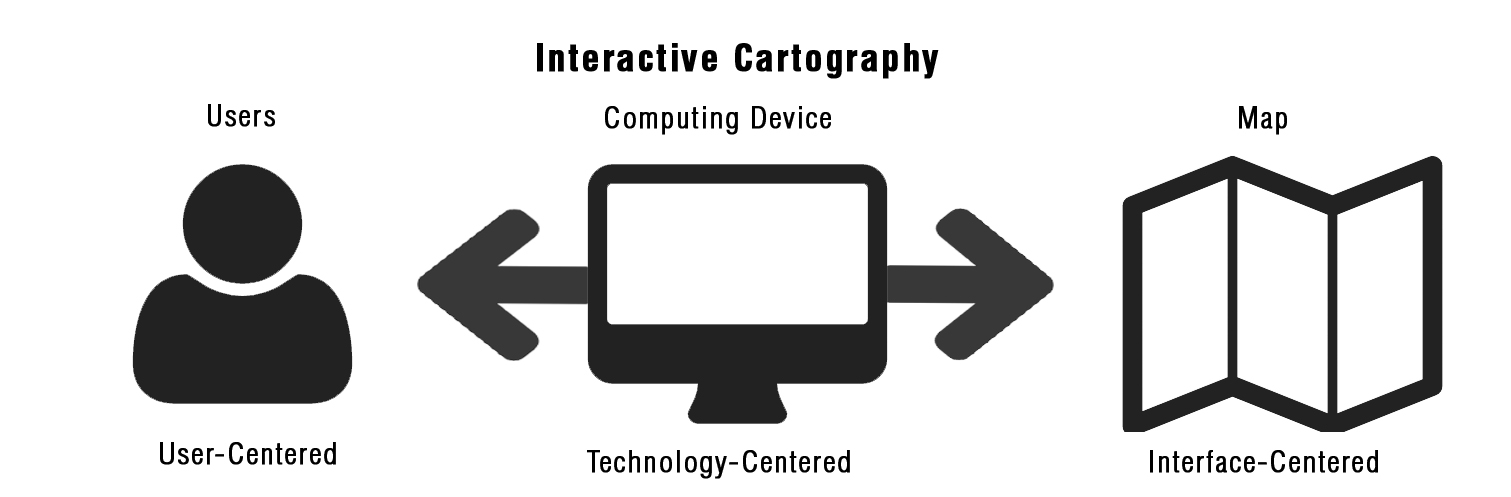
\includegraphics[width=12cm]{interactiveCartography}
    \caption{This figure illustrates the three design approaches one may adopt when developing a visualization system: User-centered, technology-centered or interface-centered. Figure reproduced from \citep[p. 64]{rothFramework}}  
    \label{fig:CartoInt}
\end{figure}

There is one more aspect to interactive cartography to consider though besides the cartographic interface and the user, and that is the computing device through which the user may interact with the map. Primarily this regards considerations in form of input capabilities, bandwidth size and processing power as well as its display capabilities. The bandwidth and processing power affect the speed at which the user interacts with the map and is therefore an important aspect of the cartographic interaction experience. Instantaneous interactions are needed to support fluid visual thinking. \citep{roth2013interactive}

\subsection{Human-Computer Interaction}

As previously mentioned, with the increase of interactive design and cartography there is additional emphasis on the needs of the user. However, of the previous technologies / visualization platform studies discussed, there has been no usability testing or user-feedback. The field of Human-Computer Interaction(HCI) deals exclusively with the interaction between the user and the system, with emphasis on user-centered design. \citep{HCI}

Although the research on web-GIS usability is scarce, there are some examples where different web-GIS have been analyzed from a very general level, looking for missing features or poor design in general. \citep{eggintoncommon} \citep{blekinge} Despite there not being much overlap in the research of HCI and GIS, the concepts of redesigning any kind of website is applicable to web-GIS as well. A common tool in the HCI community to allow for user-centered design is to let the users test the product and give feedback during the test. In one such example, researchers asked the users to give their feedback out loud as they were assigned a set of tasks to perform in the software. This way, they can more directly translate the users' opinions into the software. \citep{modeling}

Two aspects that are important to a successful design is the first impression and familiarity. The user of a system makes up its mind at first exposure, in a time frame as short as 50ms. If the users have a good first encounter with the website or product, they might ignore smaller issues occurring later. On the other hand, if the users have a bad first expression, these small issues will have a compounding negative effect. 

Familiarity for the user is also important. According to the theory of the "Mere Exposure Effect", people in general find recognizable things more attractive. \citep{zajonc} The original study is within the realm of psychology, but the effects have been proven to apply to other fields as well, such as advertising and HCI. Furthermore, repeated exposure to a product or a concept linearly increases the attractiveness of that product. \citep{hekkert}

\section{Overview of Related Technology}

\textbf{To Gyözö: Not sure what goes here for us. A discussion about modern web-GIS interfaces? Talking about openlayers? Do we discuss the current digpro systems that the users use?}

[Copied from your template]:
Relevant for engineering type of projects, where the primary aim is to \emph{construct} a prototype system, where the description of the technical details of the system components are relevant. It is important to state that in these type of projects it is also important to \emph{evaluate} the proposed system. The evaluation can be a critical analysis of the design in comparison to previous designs, but in most cases is empirical in nature where the feasibility / efficiency / scalability of the system is demonstrated by a relevant case study. 

%dpWebmap
%dpOrganizer
%dpOperator
%webGIS in general

\section{Method}

%%A Paragraph about the method in general
The method section is usually the main section of the document. It describes the method / approach in an organized way usually proceeding from higher to lower levels of detail. Thus, it is often preferred to first present the high level details of the method / approach usually as a system diagram or work-flow chart that briefly describes the general functionality and innerworkings of the components of the method / approach. Subsequent parts then in turn can present lower level details of the individual components.

\begin{figure}[H]
    \centering
        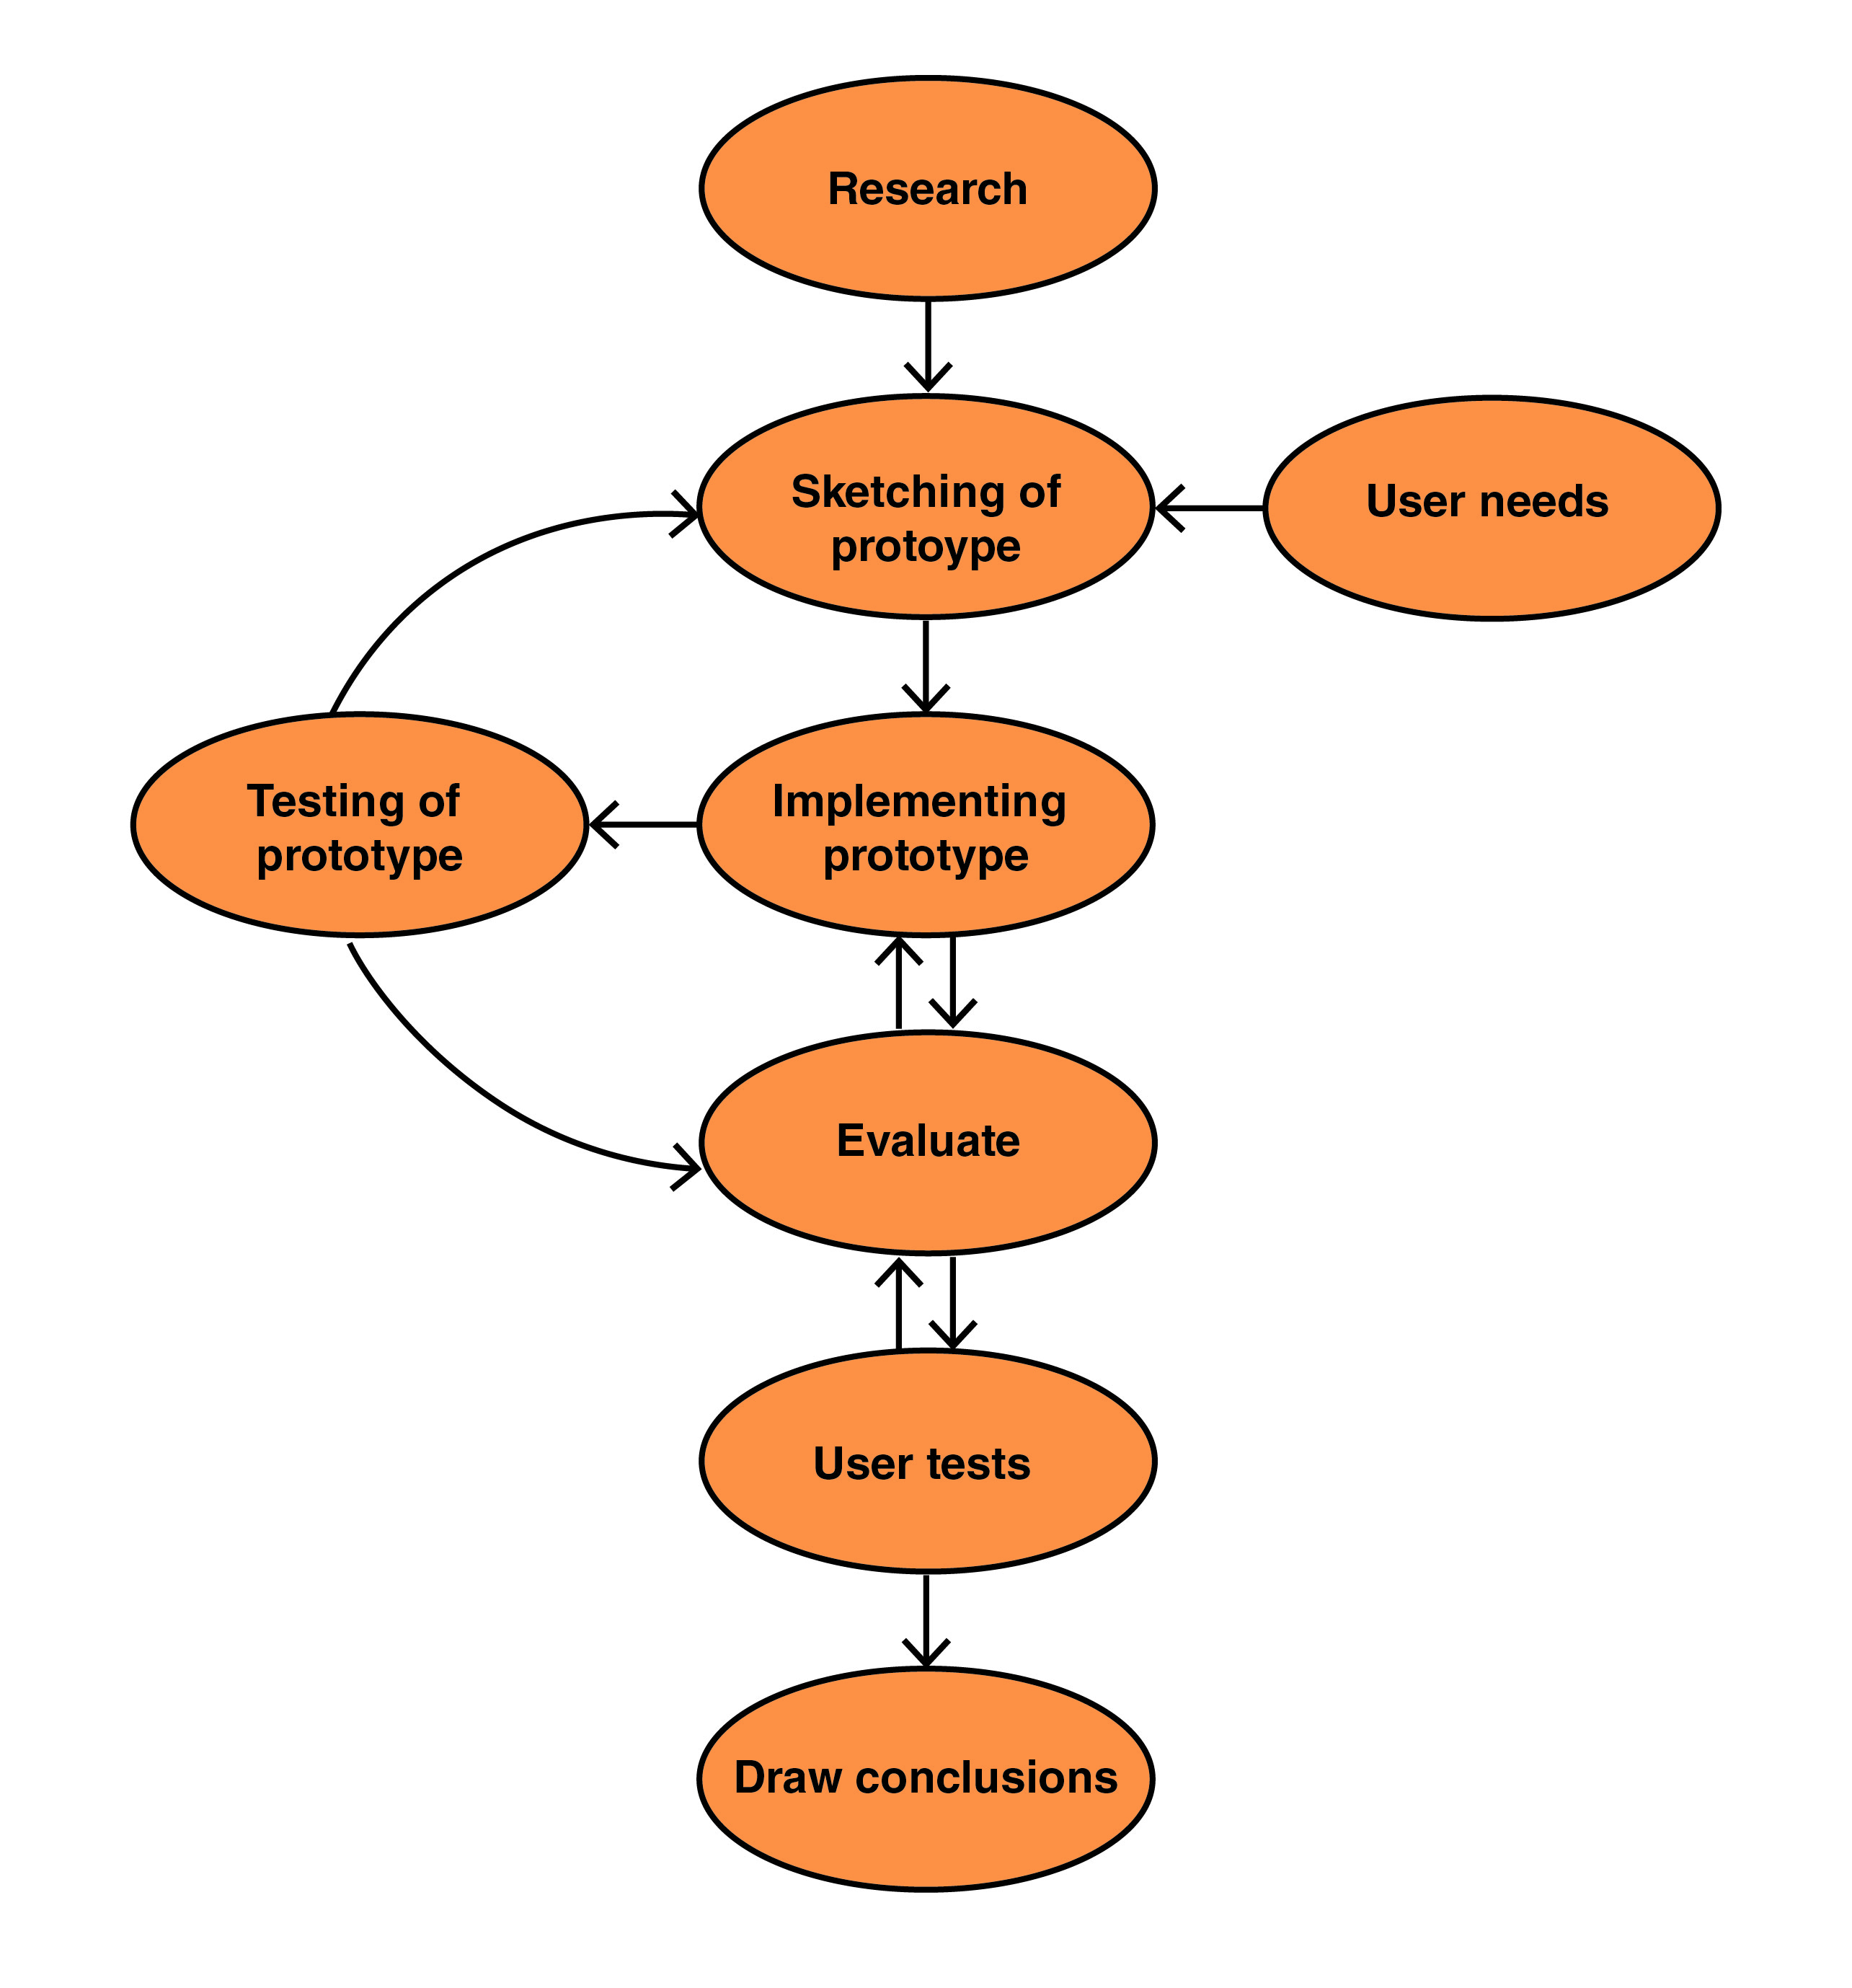
\includegraphics[width=0.8\columnwidth]{Projektplan-01.jpg}
    \caption{Flow chart overview describing the method.}
    \label{fig:Projektplan}
\end{figure}

\subsection{User needs}
%Allmänt om varför user needs är viktigt / varit i fokus? Kort?}

Since the objective of this study is to create a GIS-solution tailored to a specific type of user group one of the first things that has to be done is determine what user group to target. This decision was taken with Digpro's interest and resources in mind. It is the most practical approach since it offers the opportunity to receive instant feedback from the target user group while developing the prototype. This limitation left us with three possible scenarios, or cases, to base the prototype upon.

\begin{itemize}
    \item Case 1: Management.
    \item Case 2: Customer service.
    \item Case 3: Field work.
\end{itemize}

All of these cases are different and the user groups have different needs. However, management and customer service are slightly more alike in a technical sense. These users have the same technical characteristics, because they are working from a desktop environment and have the use of a full-sized screen, as well as a mouse and keyboard. This in contrast with the field work scenario, where the devised solution would be touched-based and designed to work on smaller mobile or tablet screens.

In addition to this, their desired functionality is somewhat similar. The customer service and management cases both require a good overview of the situation across the network, with the possibility to dive into details when needed. Conversely, the field work scenario is focused on a very small geographic area in which the work is located. 

From a technical point of view as well as from a visualization perspective it was decided that Case 2, customer service, was the most interesting to pursue in this study. However, many of the applied techniques and solutions can also be extended into the management case.

Additionally, from all the tasks that the customer service representative might have to tackle, the scope has been narrowed to focus more on an outage in the network. This scenario requires quick decision making and having information easily available, as well as provides interesting visualization challenges.

\subsubsection{Interviews}

To start the process of understanding user needs and requirements, users of the existing Digpro products is surveyed. It is imperative to not have the level of the interviews to be too technical, which means that ideally the interviews should be conducted with potential end-users of the product. Unfortunately, direct access to these users is difficult to get. However, the clients of Digpro provided interview access to their counterparts at the company. These users are not the layman users that the prototype is designed for, but more often their bosses or the person responsible for the technology at the client company.

In total, four different interviews were conducted. The first was conducted with a current Digpro employee who'd previously been responsible for the acquisition and implementation of Digpro products at his previous NIS-employer(can we name names of the companies?). Two were conducted with the current system administrator of Digpro systems, as well as the manager responsible for a specific utility, at two regional multi-utility companies. Lastly, another interview with the same setup as the previous two was held, but with an important addition. They had included one of their current employees in customer service.

The purpose of these interviews is to understand how they work with the current Digpro systems, as well as their routines and procedures when dealing with different cases and scenarios. In addition to this, it is important to gather lots of information about features that they need. Not only features that are already in the software, but also features that can be useful that are lacking. In these interviews, the interviewees were encouraged to think freely and interject at any time. 

%Beskriv hur, vilka, vad vi frågade om, när(?)}
\subsubsection{Literature}
%har vi någon litteratur på vad våra användare vill ha? tänker vi guidelines från t.ex. Umeå och/eller dokumentationen från digpros sida?}

Another aspect that complements the interviews, is to further look at the existing software to see how tasks are to be completed at the moment. To better understand that, available literature related directly to the use of the current products was studied. The first set of literature was the existing manuals to the Digpro software. By studying this, the intended work flows could be even better understood and visualized. Although the actual work flows will not be implemented 1:1 in the prototype, the intended end result and the information presented is just as important to take into account.

In addition to these user manuals, one of the utility companies interviewed provided a set of user-instructions that they used for training new users on the software. These manuals highlighted the subset of current features they used, which proved to be a very small set of all the available features. Studying these two sets of documents further highlighted some criteria that were discussed in the interviews, but also that many of the operations need to be simplified.

\subsubsection{Criteria}

After interviewing the various clients and studying the manual, the various key phrases and features were condensed into a table of criteria that were essential for a customer service solution of this kind. These criteria are presented in \Fref{tab:criteriaTable}. Although these do not represent all requests or features discussed in the interviews, they do represent the essence of what was requested.

\begin{table} [h]
\caption {Criterias gathered from the interviews and literature}
\centering
	\begin{tabular}{|l|}
		\hline
		{\bf Criteria}\\
  		\hline 
	Network map\\
    Customer information\\
    Understandable overview\\
    Access to more detailed information\\
    Search functionality\\
    Capability to communicate to customers\\
    Web-based\\
    Familiar interface\\
	\hline
	\end{tabular}
	\label{tab:criteriaTable}
\end{table}

The most requested feature, that came up in every interview conducted, is that the network map must be visible. It is key for these NIS-companies, since most if not all decisions revolve around it. The interviews conveyed that without the network map, there could be no NIS or customer service operation. Another oft-requested feature is to better integrate the customer information with the customer service platform. Although many of the tasks that the customer service representative has to deal with is payment/invoice-related, which requires systems of their own, integrating the same customer information across the different platforms will be of great help.

Further on the customer integration, a possibility to communicate outage information directly from the customer service platform. This would make one of the many different systems redundant, thus reducing the number of systems the representative has to navigate. In addition to this, good search functionality is important to quickly access information about customers, connections or to find a geographic area. This search functionality should deal with user inputs dynamically and not require and user-controlled filter, similar to the one currently implemented in the dpWebmap platform.

Since a web browser is now a commonly included feature with most operating systems, having the platform be web-based would further reduce eventual issues with software functionality, software not being installed, et cetera. Reducing the amount of specialized software that the customer service representative would need to use was a recurring theme, with a unifying web-solution a proposed solution.

One of the most frequent criticisms of the current Digpro systems is that they are simply "too much". There are lots of tools, options and plenty of information available to the user. However, this information is not always adapted to the level of the user, making it overwhelming. Therefore, default view must always be a scaled down and easy to grasp one. Since the default view is simplified, the additional information needed must be presented somewhere else. Interactivity in the map was another requested feature, where more information about an object could be shown after the user clicks on it.

Lastly, a familiar interface was also put forth as a crucial component. From the interview where the customer service employee was present, it was apparent that when the systems were perceived as too overwhelming, they would instead circumvent the problem by going to a more familiar platform. "If we can't find the customer in the map of current system, we will use hitta.se\footnote{Hitta.se is a Swedish search engine for telephone numbers, maps and addresses} instead". These kinds of familiar interfaces will also give the user a lower threshold when using the product the first couple of times, which in turn should produce a higher attraction for the product.

\subsection{Data Visualization}
%Allmänt om data visualization - stor del av visualiseringen, men inte allt
\subsubsection{Data}

Table with data

Paragraph about data

Probably paragraph about why we use such a limited area

\subsubsection{Scaling}
%Hilding
The enemy of most, if not all, visualizations, is clutter. Even the best graphic representation of an object, can be drowned out by sheer volume of objects around it. Therefore, scaling is a key concept in the visualization strategies employed for the high-volume datasets. These include connection points, where the network connects to the customers' houses, and all the arcs that make up the network.

Scaling means that the amount of data displayed for the user depends on the resolution or the zoom level. Instead of displaying all of the data all the time, the system is designed to show more details in the network as the user zooms in. The different utilities divide their network somewhat differently, but in general there are three categories of arc type. These three different types are listed in \Fref{tab:arcs}. Since most of the utility networks used in the program is laid down beneath the road surface, i.e. it closely follows the shape and characteristics of a road network, a road network equivalent is also provided.

\begin{table} [h]
\caption {Arc types}
\centering
	\begin{tabular}{|l|l|l|}
		\hline
		\bf Arc type & \bf Example & \bf Road network equivalent\\
  		\hline 
		Main & From a substation to neighborhoods & Main roads\\
		General & From the main arc to the neighborhood. & Generic roads \\
		Service & From a general arc to the customer. & Driveways and small streets\\
		\hline
	\end{tabular}
	\label{tab:arcs}
\end{table}

At much of the less detailed zoom levels, i.e. the bigger levels, there is no point to show anything other than the main arcs. Conversely, the service arcs need only be displayed at the most detailed zoom levels, when the individual houses are discernible. Finally, the general arcs are added at a rather early stage, when transferring from a more regional to a local view. These settings will ultimately vary depending on the geographical extent of the network. Having more than three classes of attributes will also enable a more fine-tuned scaling, but that was not present in any of the networks included in this study.

An attempt was made to determine the scaling levels on connectivity instead of a set of attributes. The theory behind this being that more connected arcs are more crucial, therefore meaning they should be shown at a higher zoom level. However, since the utility networks most commonly featured in NIS often follow the road network, this does not produce the desired result. Since the connectivity in a road network is decided by the amount of roads going into an intersection, assuming one node for each intersection, the connectivity-approach produces 

%Snygga till slutet här

\subsubsection{Clustering}

Another way of reducing the data amounts displayed is by applying clustering algorithms. There is no shortage of clustering algorithms, with varying levels of complexity, available in the field. Despite variations in applications and approaches, they all strive to accomplish the same task: aggregating the data based on a set of properties, such as distance or type.

The first type of clustering is a simple distance-based cluster, where all points that fall within a certain radius are aggregated and displayed as a group of points, usually at the center of the clustered points. A crude example of purely distance-based clustering is displayed in \Fref{fig:Cluster}

\begin{figure}[H]
    \centering
        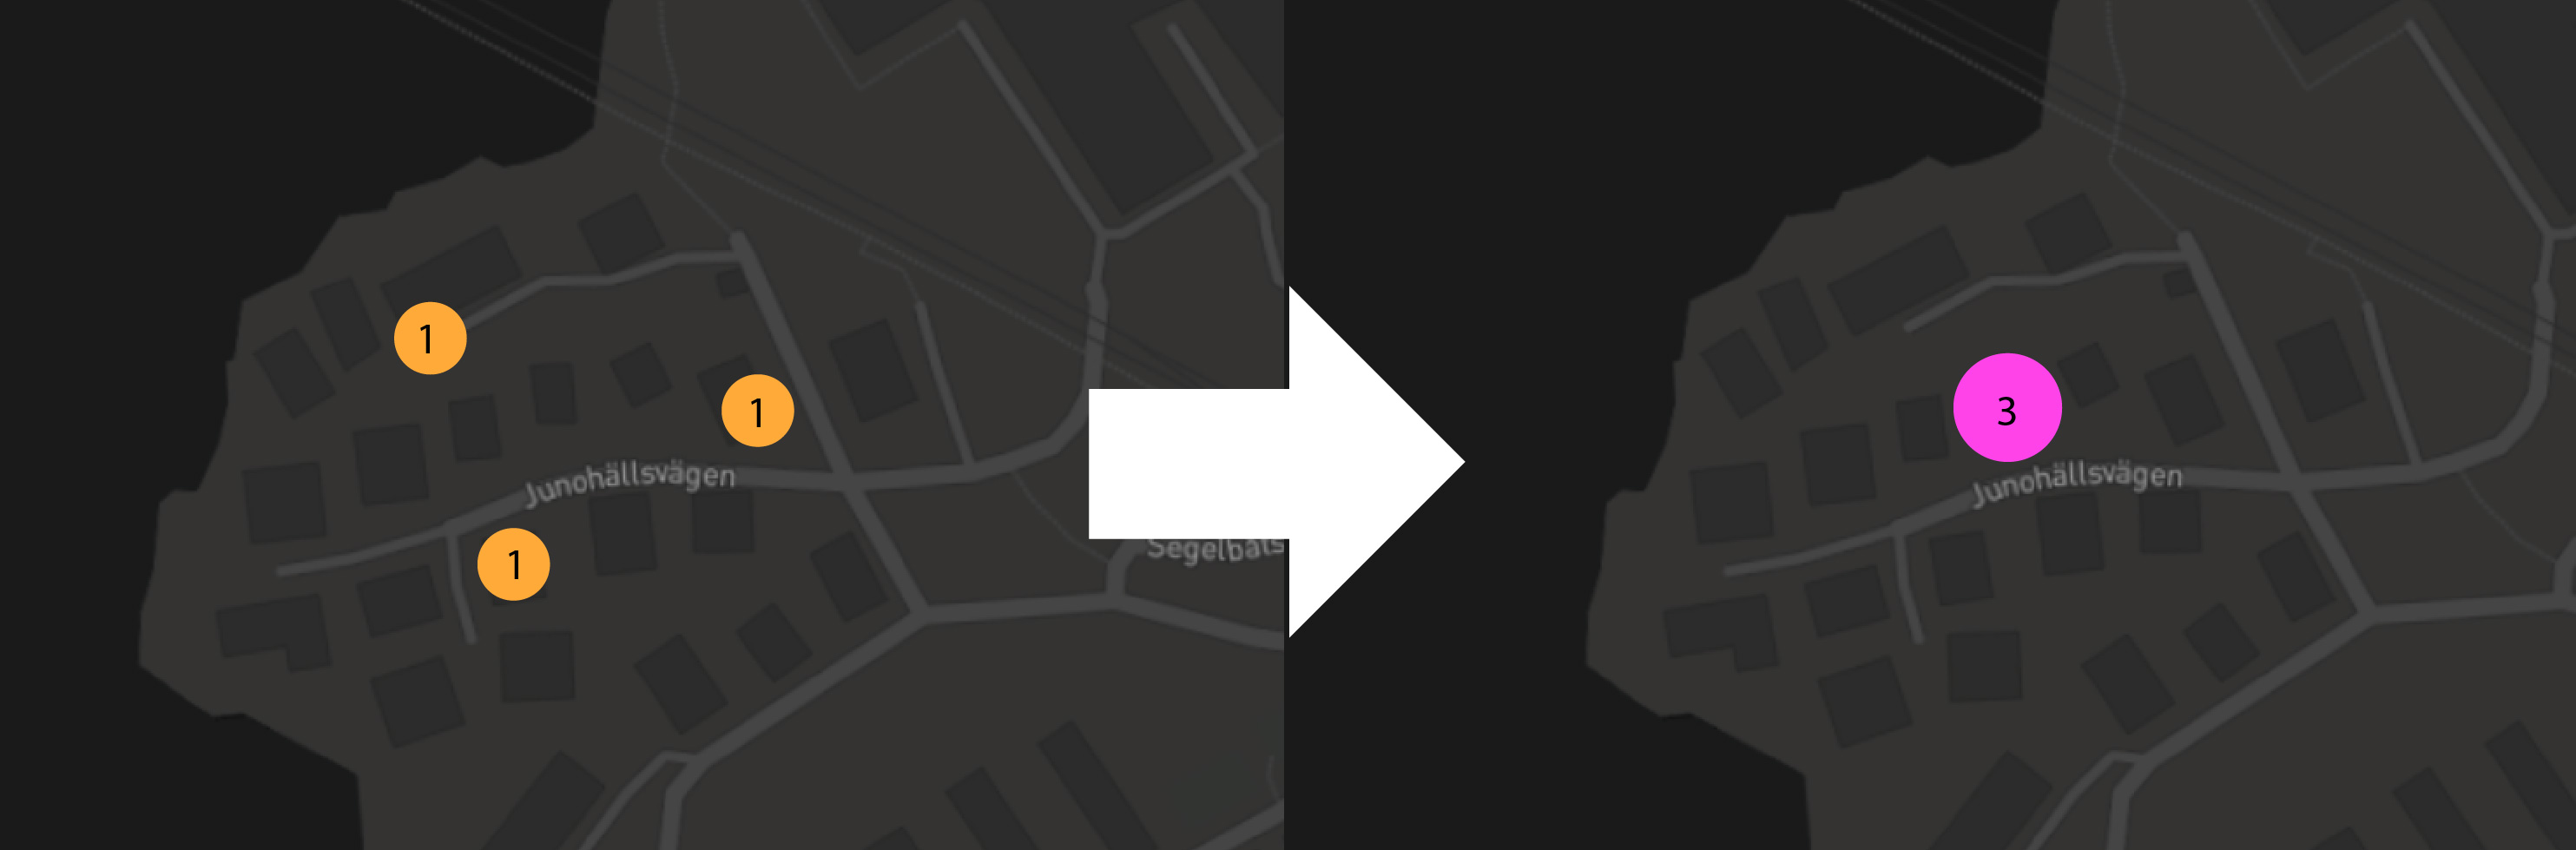
\includegraphics[width=12cm]{Kluster-01.jpg}
    \caption{An example of a cluster}  
    \label{fig:Cluster}
\end{figure}

However, if this method is applied to several outages across different utilities, the desired effect is not achieved. Since most outages are utility-specific, clustering all the points (from multiple utilities)

How to implement clustering based on "attributes"?

Better to cluster all and show distribution, or better to cluster per utility?

\subsubsection{Line objects}

In the prototype the networks are represented by line segments. Each network line segment has its own unique type of style. Beyond having their own distinct color associated with them, the lines themselves have different styles in the sense that some are dashed or dotted. This further helps distinguish the lines from each other in cases where it may be hard for the user to separate color combinations in cases of line intersection.

When assigning colors to the different utilities no special consideration was taken to what may be associated with a special color, with one exception. There is a Swedish standard for water lines that demand that water lines should be represented by a blue color. The only considerations otherwise when choosing color was to choose colors that have as much contrast as possible when compared to each other, and to avoid certain color combinations that are particularly difficult for color blind to distinguish between. However, internally within a company there may be standards regarding colors and utilities and they should then of course be followed.

In terms of visualization, another important aspect of the line segment style is the thickness of the line. If the line is too thin it will be hard to discern. In this prototype the thickness of the line segment was also used as a way to emphasize parts of the network that suffers from an outage. The line segments that are affected are then thicker than the rest of the network. Instead of using thickness it was also considered using stroke to highlight affected parts of the network in order to distinguish them from functioning parts.

\subsubsection{Point objects}

Connections, customers, repairs and installations are represented as point objects in the map. Connections are actual points while customers, repairs and installations are symbolized by icons

How does one represent a point? Icons, do they help?

\subsubsection{Background map}
%Ella

\subsubsection{Heatmap}
%Ella
Heatmaps! Looks great, contains very little information

%We also included a heatmap layer in our prototype representing 

\subsubsection{Interactivity}

\subsection{Prototype}

In order to verify if tailoring a visualization system to the needs of a specific user group is feasible a prototype was created. The development of the protoype was carried out in several different steps, as shown in \Fref{fig:Projektplan}

\subsubsection{Mock-ups}

Before starting to actually implement the prototype, a few mock-ups were made. These are based on the previously acquired information from literature and interviews. The interface design of the mock-ups is inspired by Digpro's product dpWebmap, as well as the interface of Google Maps. This is because there is value in giving the prototype an interface the user feels accommodated to, thereby making it more intuitive and less confusing. A specific request from the interviewees was also that the interface is simple, intuitive and without any unnecessary elements in form of tools or menus, which serves more as a distraction than a benefit.

\begin{figure}[H]
    \centering
        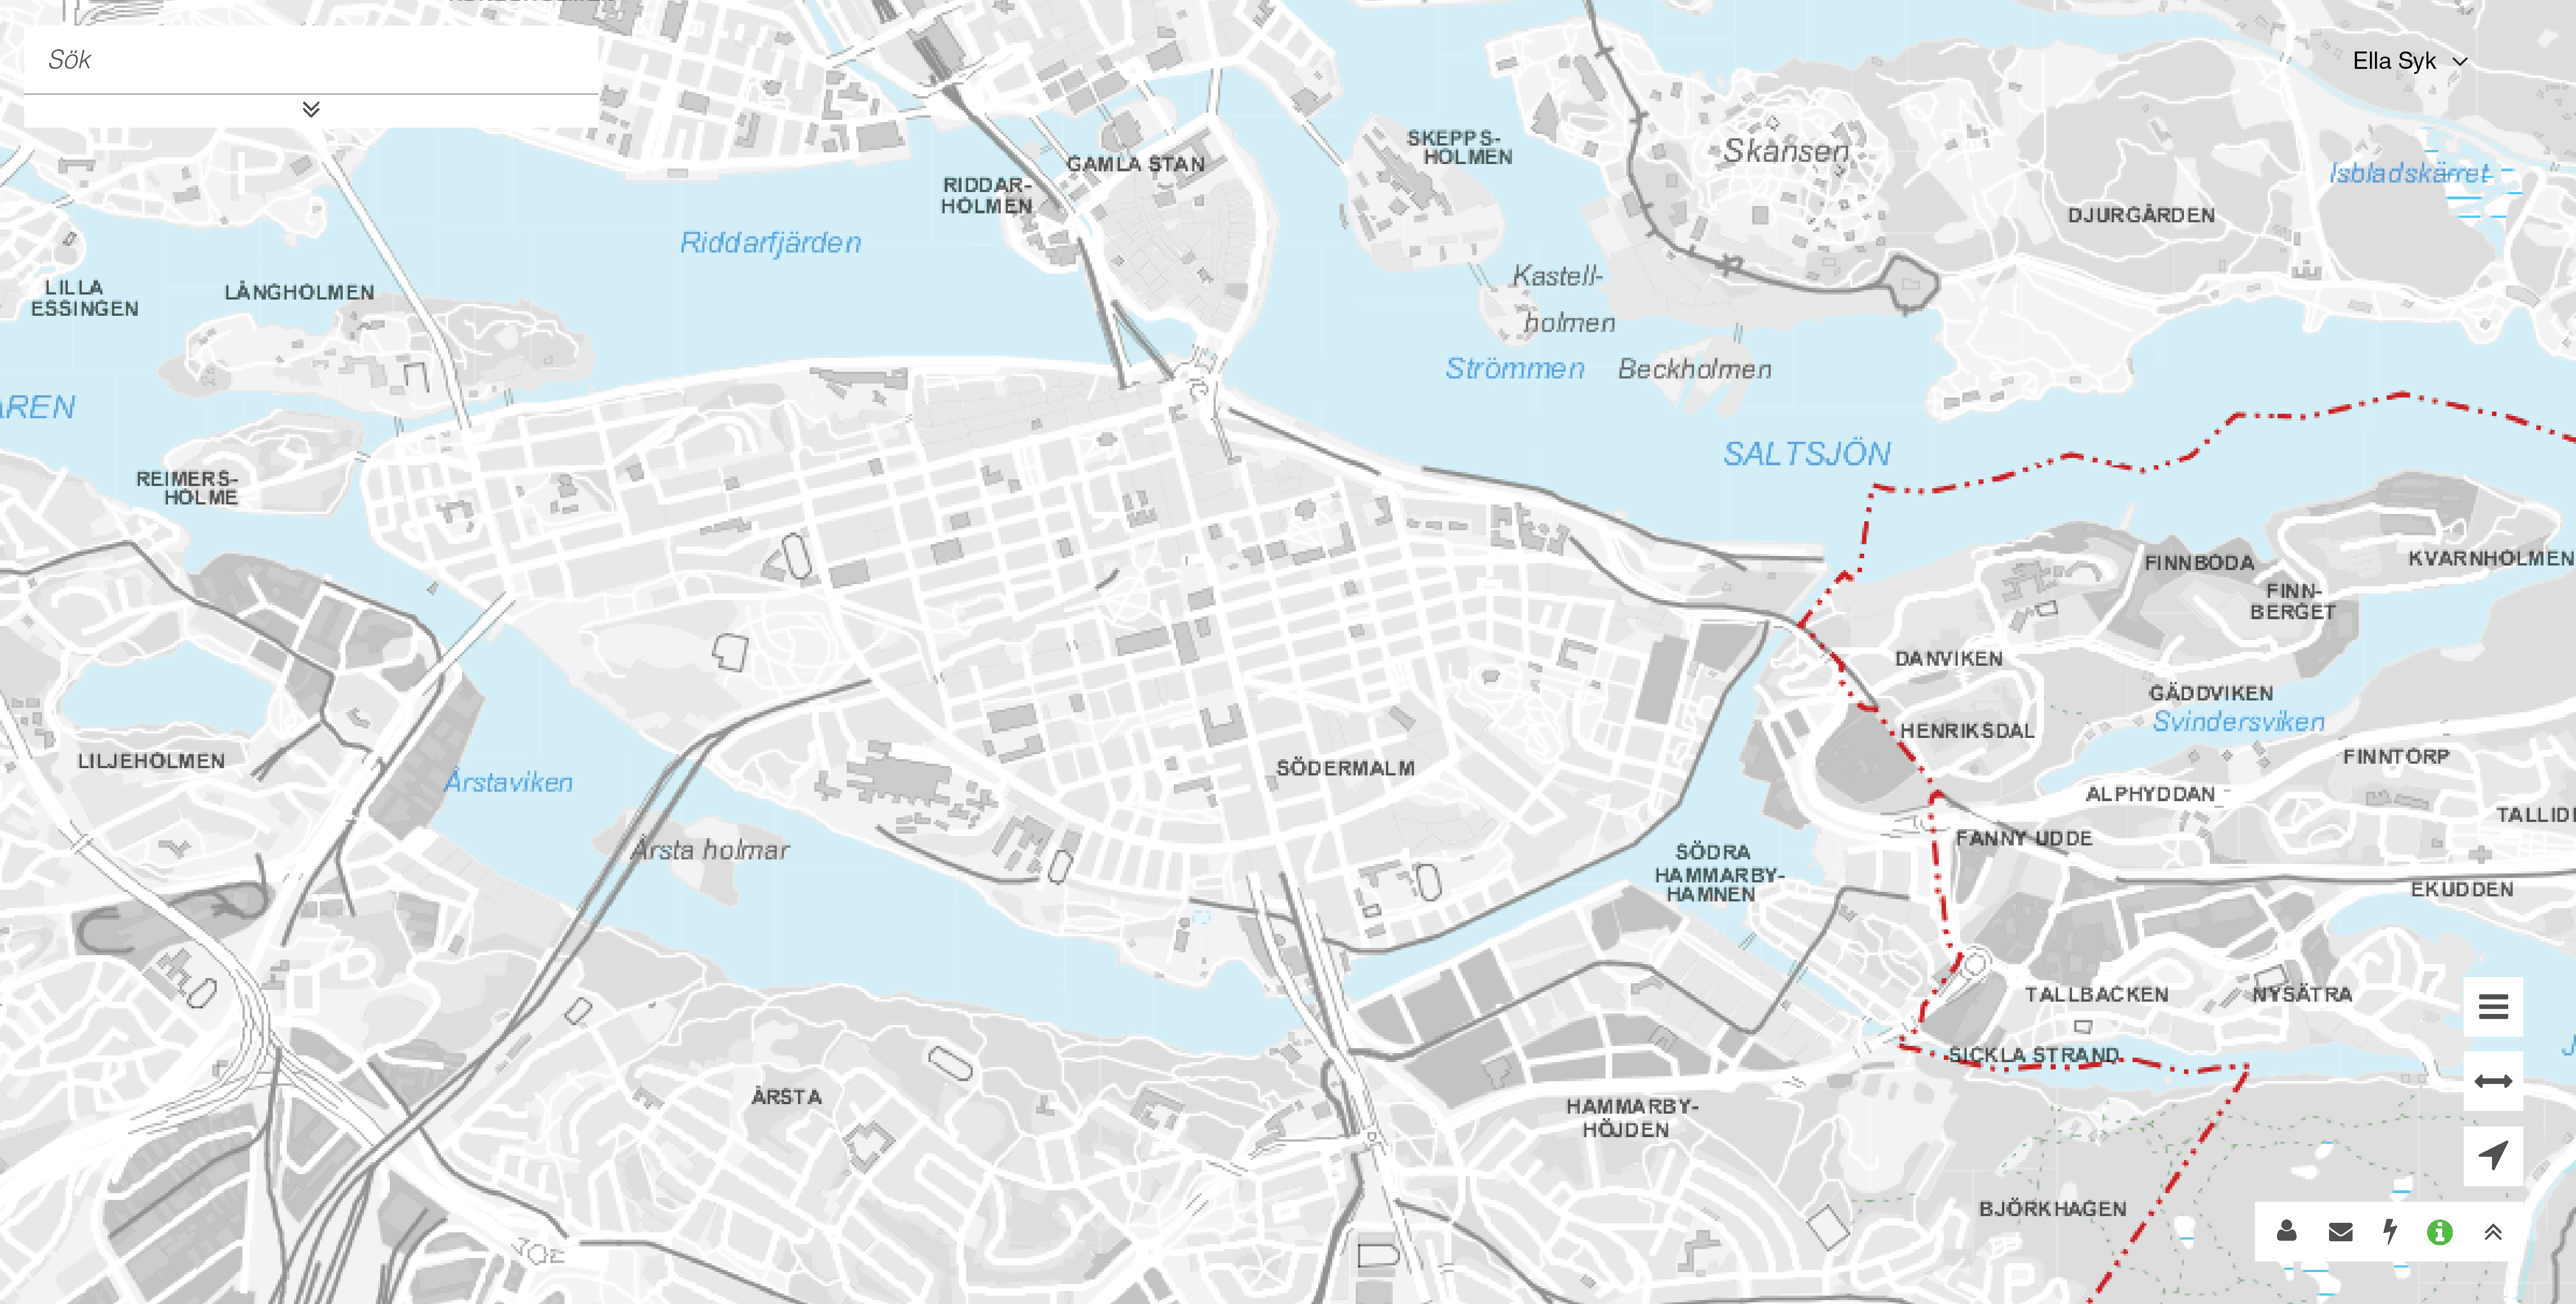
\includegraphics[width=15cm]{mockup.jpg}
    \caption{One of the mock-up images depicting the start screen of the prototype.}  
    \label{fig:Mockup}
\end{figure}


\begin{figure}[H]
    \centering
        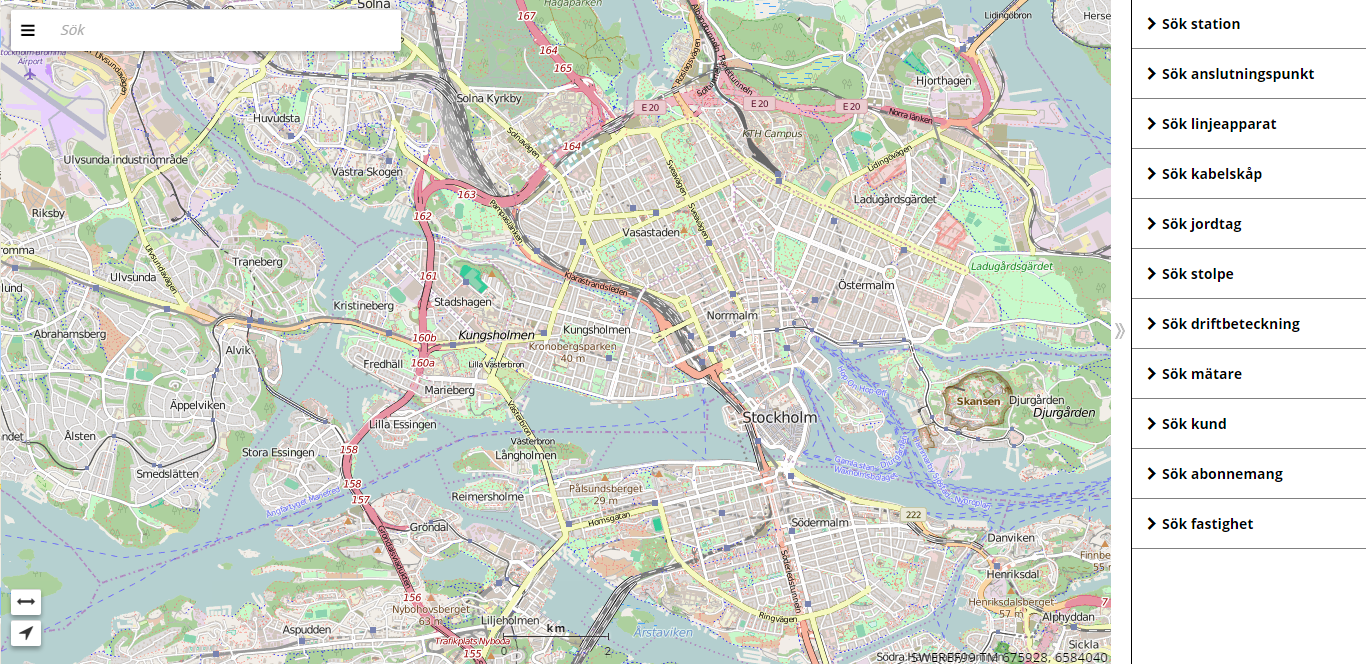
\includegraphics[width=15cm]{dpwebmap.png}
    \caption{Screenshot of the dpWebmap application start screen.}  
    \label{fig:dpwebmap}
\end{figure}


\begin{figure}[H]
    \centering
        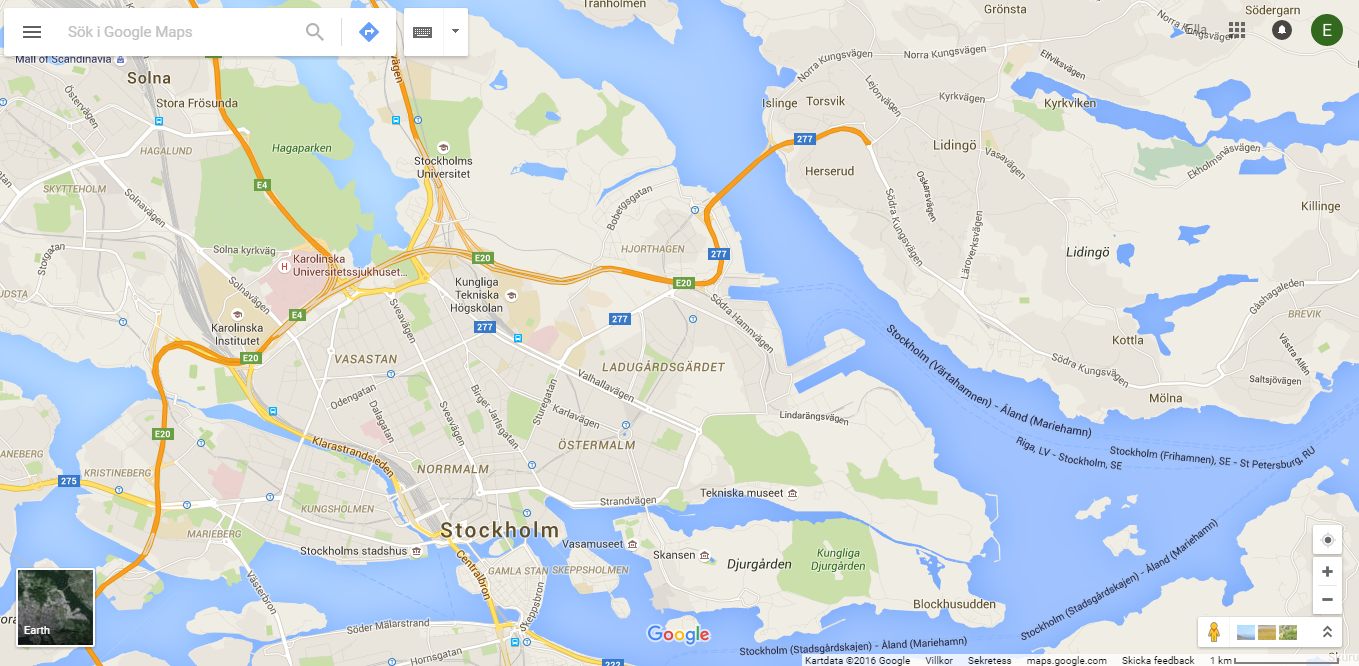
\includegraphics[width=15cm]{googlemaps.png}
    \caption{Screenshot of Google Maps start screen.}  
    \label{fig:Googlemaps}
\end{figure}

As shown by \Fref{fig:Mockup}, \Fref{fig:dpwebmap} and \Fref{fig:Googlemaps} there are similarities between all of them, such as the design and placement of the search bar. In the toolbar in the lower right corner of \Fref{fig:Mockup} there are some special features, that are of specific use to the users in this case study. The user icon provides easy access to information about customers that are affected by an outage. The envelope icon gives access to a messaging service so affected customers or field workers can be immediately informed if need be. Finally, the round information icon triggers a status report which contains a summary of what is going on in the map in regards to installations, repairs and outages. These are all features that were requested by the interviewees.

The mock-ups were made using Adobe Illustrator and were presented to several persons, among them some of the interviewees as well as some Digpro employees. Based on their feedback, the mock-ups were then evaluated and modified accordingly. 

\subsubsection{Implementation}

To facilitate evaluation of the previously discussed visualization techniques, and by extension help to answer the research questions, the concepts all had to be implemented into a web-based prototype. 

\subsubsubsection{Technologies}
%Hilding - om openlayers
HTML5 is the newest revision of the HyperText Markup Language, HTML for short. It includes a wide range of new features, aimed at replacing many proprietary plug-in technologies, such as Flash or Silverlight. \citep{webGIS} HTML is supported by most major browsers, which in term provides a platform- and plugin-independent solution that works right out of the gate. 

In addition to HTML5, "JavaScript is one of the 3 languages all web developers must learn"\citep{w3JS}. JavaScript is a powerful web-development language that controls much of how websites function. With lots of libraries, JavaScript is a versatile language well-suited for many web-development tasks. One such library is the open-source mapping-centered library OpenLayers, with its current 3rd major version OpenLayers 3. The dpWebmap products of Digpro currently use the older OpenLayers 2, which shares much functionality with its more modern counterpart.

OpenLayers is not something the user needs to install, but is rather acquired via the web when the request is made to the website. It is also supported by most modern browsers, further ensuring platform independence. OpenLayers contains a large amount of functions for presenting, manipulating and interacting with geographic data. It supports common geographic formats such as KML and GeoJSON, plus web-based formats like Web Map Service (WMS).

\textbf{To Gyözö: Do we need to source the stuff above? It's hard to find anything, other than linking to the documentation of the functions, which seems like the wrong approach. \\ \\ Also: as previously asked, should this be moved to the related tech-part?}

\subsubsubsection{Front End}

Interface, CSS

Features

\subsubsubsection{Back End}

Along with the front end features, there is also a back end component of the prototype. Firstly, there is a PostGIS spatial database in which the geographic data is stored. This is in substitute of the real database system that a NIS-company usually would have. In this database, information about customers as well as the network itself, is efficiently stored. Although the storage does not mirror the more complicated database structure of the Digpro systems, they preserve the same relationship between the arcs, nodes and customers that can be expected in a NIS.

Another substitute is the functionality that simulates an outage in the network. In reality, this information is automatically provided from systems specific to the utilities. These Supervision, Control and Data Acquisition (SCADA)-systems automatically report when outages occur in the network. \citep{avbrott} However, linking these systems to the prototype is quite difficult, which meant an alternate solution was desirable. The solution is to have the operator input a node-ID, after which it checks all the neighboring nodes. If there's a path from that node to the substation that does not include the node selected by the user, it is safe. Otherwise, if the only way to get from the neighbor to the substation is to go via the selected node, that node is now considered to be broken. The practical effect of this solution is that only parts of the network that are not redundant can have outages simulated in them. 

\subsection{Testing and feedback}
%Beskriv vikten av testing / feedback
\subsubsection{Quantitative}
%Hur tar vi fram den kvantitativa datan? Varför?
\subsubsection{Qualitative}
%Hur tar vi fram den kvalitativ datan? Varför?
\subsection{Evaluation}
%Hur skiljer det sig från testing and feedback? Repetition?
\subsubsection{Survey}

\subsubsection{Presentation}

\section{Results}
%Beskriv de resultat som vi i dagsläget inte har

\section{Analysis}

%Analys av sagda resultat

\section{Discussion}

%Diskussion

%diskutera resultat utifrån vårt case

%diskutera resultat utifrån världen/generellt

%Finns det några generalla riktlinjer vad gäller kartografisk gränssnitt design? Kan man dra nytta av existerande gränssnitt? hint google

%Finns det värde i att skräddarsy kartors gränssnitt? Är det värt det sett till praktiska kostnaden att anpassa det? vad behöver skräddarsys, kartan och det som visas i eller gränssnittet?

%anpassa kartan mer efter zoomnivå vad gäller detaljer - oftast anpassas bara bakgrundskartan. men som feedback från vårmötet samt related twerk pekar på så bör även tematiska lager anpassas

%kunna justera opacitet av lager som användare

%trycka på vad som är viktigt med att anpassa kartan - att kunan få en lättförståelig överblick över vad som pågår oavsett vem i projektgruppen man är är användbart inte bara vid avbrottshantering utan även i byggprojekt etx. Beslutsunderlag

%Karta behövs som komplement till tabeller, man kan upptäcka mönster

%diskutera feedbacken från vårmötet

%Diskutera och jämför med feedback från formulär

%att användaren (inte alla användare) har möjlighet att påverka hur saker representeras - pros/cons

%Färgblindhet och associationer till färger och symboler

%problems we have encountered

%cluttered interface problem
%CLuttered interface - compare with digpro java client interfaces and talk of interviews

%klustring av nätverk!

%webgis - gis är nu lätttillgängligt men inte standardiserat. som visas på i litteraturstudien har SIS påbörjat ett arbete att ta fram riktlinjer för webbkartor och det sker idag, finns alltså inte så mycket sen tidigare. Prata om APple maps och dess initiala release!

Visualization today is not only about what is actually visible graphically in the map, the interactivity lends another dimension to visualization as well. Partly through the possibility to activate and deactivate layers but also through pop ups and clickable graphics, to mention a few examples. The interactivity enhances the graphical presentation and enables more solutions for displaying data in an organized and uncluttered manner.

\subsection{Future research}

%Ta med lite idéer från powerpointen, samt prata om användarcentrerad design i allmänhet. Viktigt med en bra slutkläm - samt viktigt att inte fokusera för mycket på digpros scenario, utan hålla det generellt.


\newpage
\bibliographystyle{apacite}
\noindent
\bibliography{newbib}

\end{document}
